\documentclass[12pt,a4paper]{article}

% Packages
\usepackage[margin=1in]{geometry}
\usepackage{amsmath, amssymb}
\usepackage{bm}
\usepackage{graphicx}
\usepackage{fancyhdr}
\usepackage{lastpage}
\usepackage[section]{placeins}
\usepackage{siunitx}
\usepackage{xfrac}
% Header and footer settings
\pagestyle{fancy}
\fancyhf{} % Clear all header and footer fields

% Header
\fancyhead[L]{EASC3404}
\fancyhead[C]{Lab 2}
\fancyhead[R]{Structural Geology}

% Footer
\fancyfoot[C]{Page \thepage\ of \pageref{LastPage}}

% Header and footer line
\renewcommand{\headrulewidth}{0.4pt}
\renewcommand{\footrulewidth}{0pt}

% Remove header from the first page if needed
% \thispagestyle{empty}

\begin{document}

% Title (optional)
\begin{center}
    \Large\textbf{Finite Strain Analysis and Shear Zones}\\[0.5em]
\end{center}


% Lab instructions
\section*{Question 1 (in class)}
We have derived the $\bm{F}$ matrix for the pure shear deformation in class.
Now derive the $\bm{F}$ for sinistral simple shear deformation with a shear strain of $\gamma = \tan\theta$.
Show your reasoning. 
The following diagram of sinistral simple shear deformation is provided to you as a reference:
\begin{figure}[hbpt!]
  \centering
  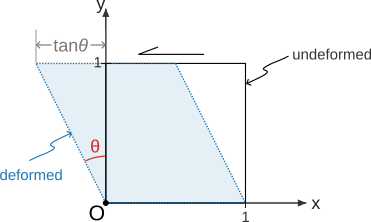
\includegraphics{simple_shear.pdf}
\end{figure}



\section*{Question 2 (in class)}
Rerun the \texttt{finite\_strain\_analysis.ipynb} with your derived $\bm{F}$ for 
the sinistral simple shear with increasing shear strain, 
from $\theta = $ \SI{30}{\degree} to \SI{60}{\degree}. 
Show figure outputs from the \texttt{Jupyter} notebook and briefly explain:
\begin{enumerate}
  \item Why simple shear deformation is considered as \emph{non-axial}?
  \item What is the sense of rotation of the material lines? 
    Are there any materials lines that are not rotated at all?
  \item Are material lines experiencing shortened at $\theta = \SI{30}{\degree}$
    still under shortening as we accumulate shear strain and reach $\theta = \SI{60}{\degree}$?
\end{enumerate}


\section*{Question 3}
The following figure displays a narrow shear zone developed in a magmatic rock.
Now let's do some ``forward modelling'' on a virtual piece of rock sample.
Plug the $\bm{F}$ you computed in Question 1 into \texttt{homogeneous\_strain.ipynb}. 
Experiment with different shear strain ($\gamma$) values, do the modelled strain ellipsoids 
produce the similar deformation pattern as the natural shear zone in the figure?
\begin{figure}[hbpt!]
  \includegraphics[width=\linewidth]{shear_zone_field_photo.pdf}
\end{figure}


\section*{Question 4}

\begin{figure}[hbpt!]
  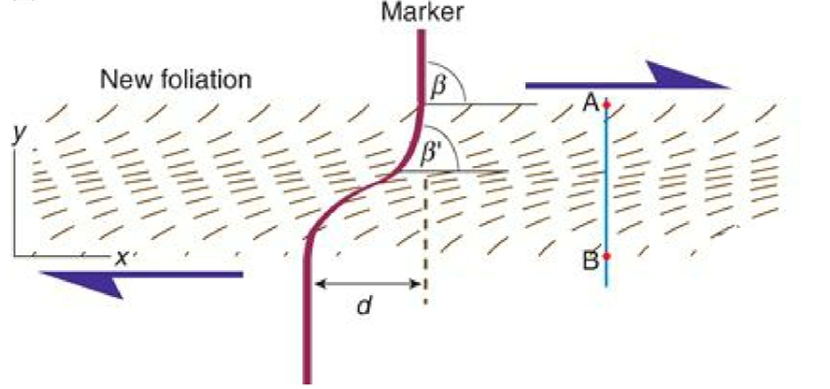
\includegraphics[width=\linewidth]{measurement_method.png}
\end{figure}
\begin{enumerate}
  \item Create two shear strain profiles, A and B, across the shear zone. 
    On the transparent paper, mark at least 8 oblique fabrics along each profile and 
    measure the angles ($\beta$) between the foliation and the shear zone boundary.
    Record the position and $\beta$ angle of the measurements.
  \item Average the measurements along both profiles and input the values into 
    the notebook file \texttt{heterogeneous\_strain.ipynb} 
    to construct a spatially varying shear strain $\gamma$ profile.
    The $\beta$ values has the following relationship with the shear strain $\gamma$:
    $\gamma = \sfrac{2}{\tan 2\beta}$ and is already implemented for you in the notebook.
  \item Compute the overall displacement $d$ (\unit{\cm}) of the shear zone along each profile
    using the following relationship: $d = \int_{-2}^{2} \gamma d\gamma$. \\
    (Hint: consider using the function \texttt{scipy.integrate.simpson} )
  \item Show the modelled deformation pattern from the figure. 
    Is it more realistic than the previous model? 
    What does that tell you about the strain distribution within the shear zone?
\end{enumerate}

\end{document}
